\documentclass{article}
\usepackage[utf8]{inputenc}

\title{CTA200H - Final Project}
\author{Louis Branch}

\usepackage{graphicx}
\usepackage{amsmath}
\usepackage{amssymb}
\usepackage{cancel}
\usepackage{mathabx}
\renewcommand{\thesubsection}{\thesection.\alph{subsection}}
\pdfpkresolution=300
\usepackage{geometry}
 \geometry{
 a4paper,
 left=10mm,
 right=10mm,
 top=10mm,
 bottom=10mm
}

\date{May 2022}
\setlength{\parindent}{0em}
\setlength{\parskip}{0.5em}
\renewcommand{\baselinestretch}{1.1}

\begin{document}

\maketitle

\section{Pulsar Profiling}

Neutron stars have strong magnetic fields that emit beams of radiation from 
their magnetic poles. As the star rotates over its spin axis, the radiation beam
is seen once for every rotation when an observer becomes aligned with the 
star's magnetic axis.

From the point of view of an observer, the star's brightness is increased many
folds during this short period, creating a distinct pulse, hence the name
pulsating star, or pulsar. However, because the star's rotation and magnetic
axes can have different alignments, the observed brightness varies during the
precessional motion of the star.

In this project we use computational techniques to simulate and plot a pulsar
profile in which its observed brightness follows the von Mises distribution,
a continuous probability distribution on a circular plane with a range from 0
to 2 $\pi$.

\begin{equation}
I(\phi \, | \, \mu,\kappa) = I_{peak}e^{\kappa\, cos(\phi-\mu)}
\end{equation}

Where:

$\phi$ is the pulsar phase which depends on its angular frequency

$I_{peak}$ is the peak observed brightness

$\mu$ is the mean direction of the distribution ($0 \leq \mu \leq 2 \pi$)

$\kappa$ is the concentration parameter, the reciprocal of dispersion,
defined as:

\begin{equation}
\kappa = \frac{log \, 2}{2\, sin^2(\pi D/2)}
\end{equation}

When $\kappa = 0$ the distribution is uniform, but for a pulsar its
concentration value depends on $D$, the duty cycle. The duty cycle is the ratio
of pulse width to the period of repetition of the pulse.

Examples of duty cycles of detected pulsars (Henry and Paik, 1969):

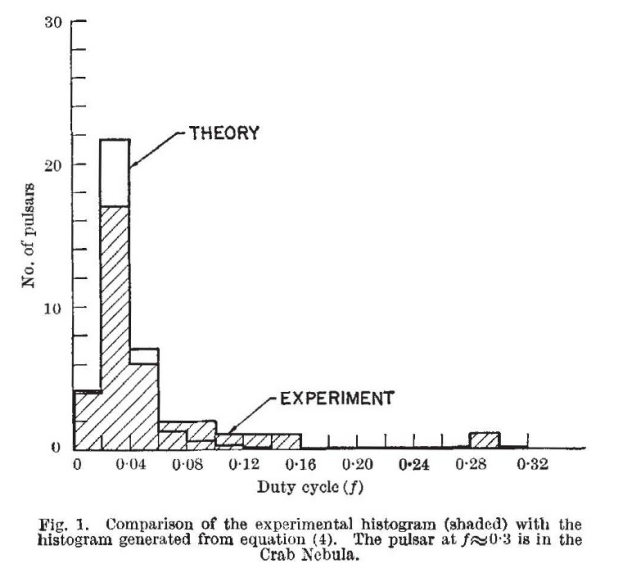
\includegraphics[scale=.45]{dutycycle.png}

\subsection{Simulation Constants}

For this project we use the following constants for the observed intensity
function:

\begin{align*}
    \phi_{0} &= 1 \\
    I_{peak} &= 100\\
    \mu &= 1\\
    D &= 0.1\\
    T &= 10 \, ms 
\end{align*}

\section{Simulated Brightness Time Series}

Using the scenario constants we simulate a time series from 0 to 2s with 200Hz
sample rate, twice the pulsar angular frequency.

The first plot shows the entire 2s period in which we can see the observed
brightness varying sharply from its peak $\approx 1.4 \cdot 10^8$ to zero.
Therefore, from an observer the pulse increases by 8 orders of magnitude when 
the beam is in phase.

The next plot shows individual pulses at its highest and lowest observed
brightness. From the first image we can see one pulse for each rotational period
(0.01s).

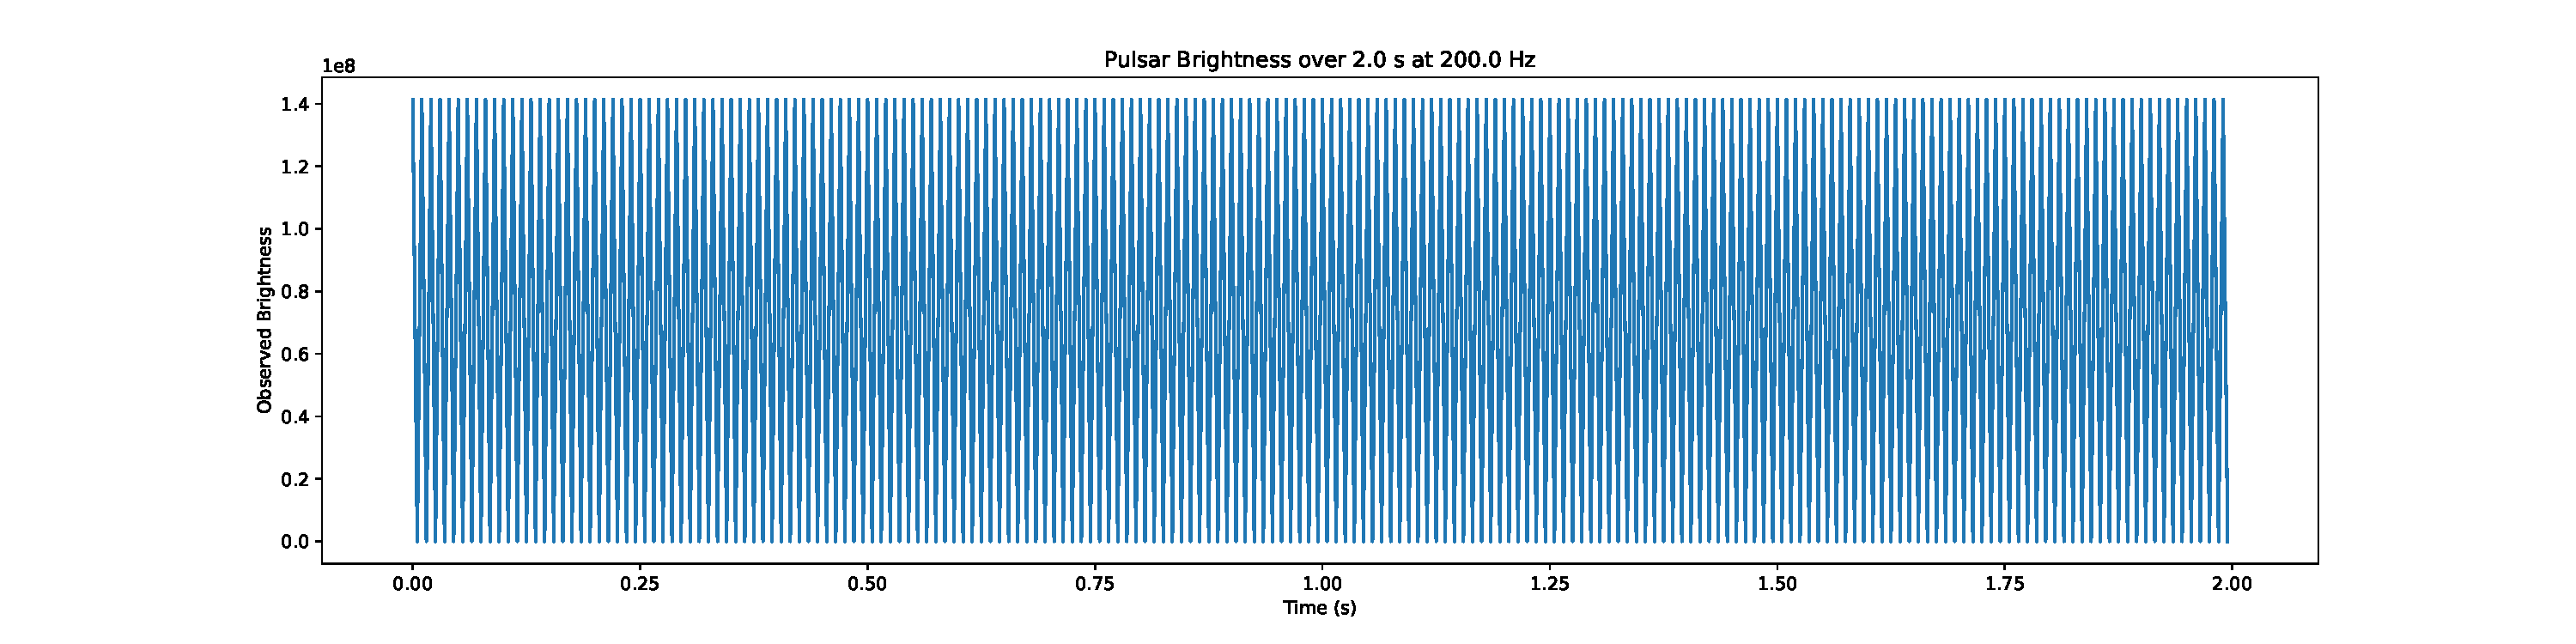
\includegraphics[width=\textwidth]{brightness_200.0_hz.pdf}
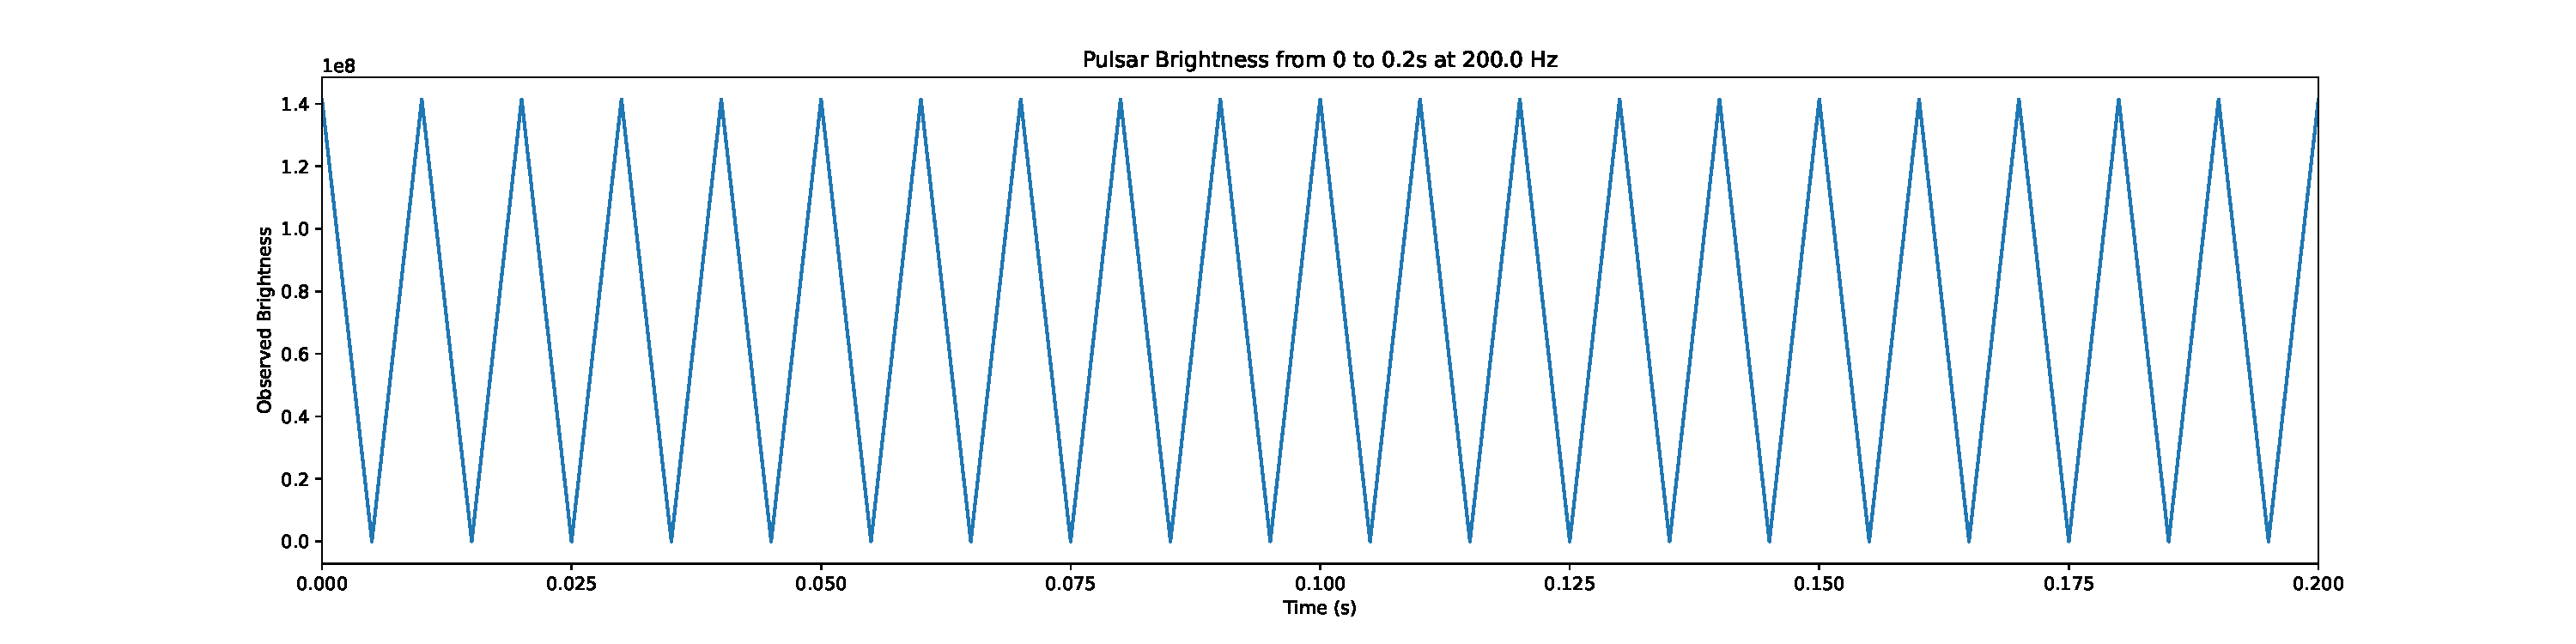
\includegraphics[width=\textwidth]{brightness_200.0_hz_range.pdf}

Using different sample rates over the same period it is possible to see how
constructive and destructive interference patterns affect the signal. When
sampling at 180 Hz instead the signal becomes less clear since the detection
is out of phase.

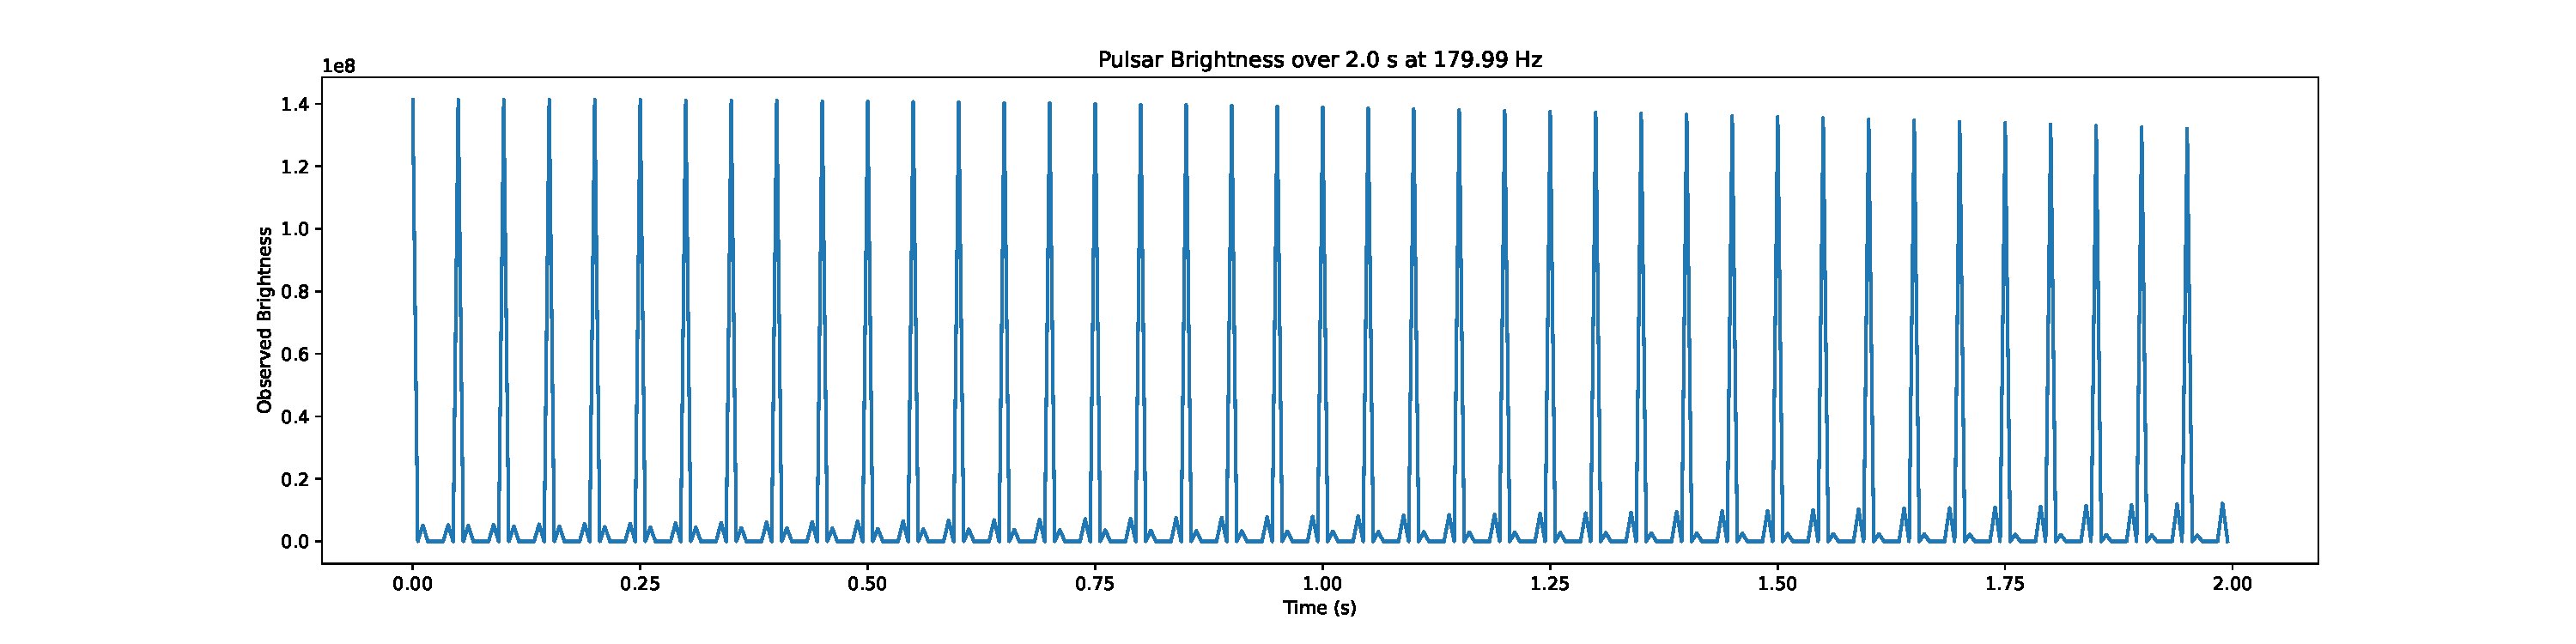
\includegraphics[width=\textwidth]{brightness_179.99_hz.pdf}
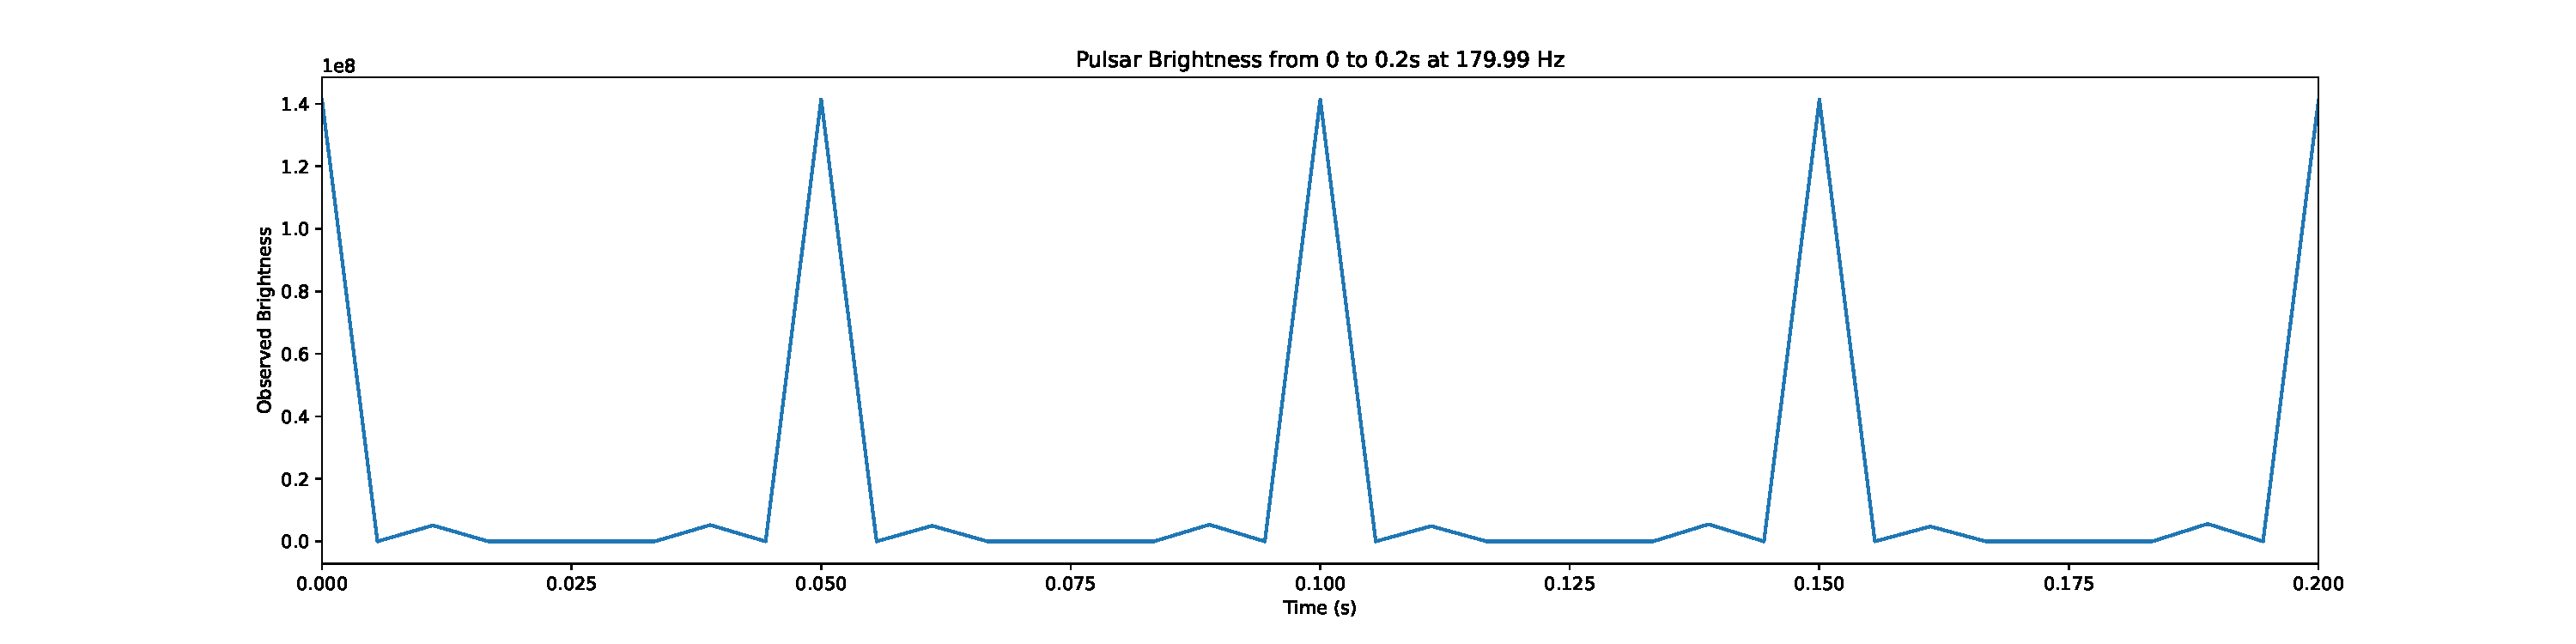
\includegraphics[width=\textwidth]{brightness_179.99_hz_range.pdf}

A sample rate of 100Hz or below produces a continuous signal.

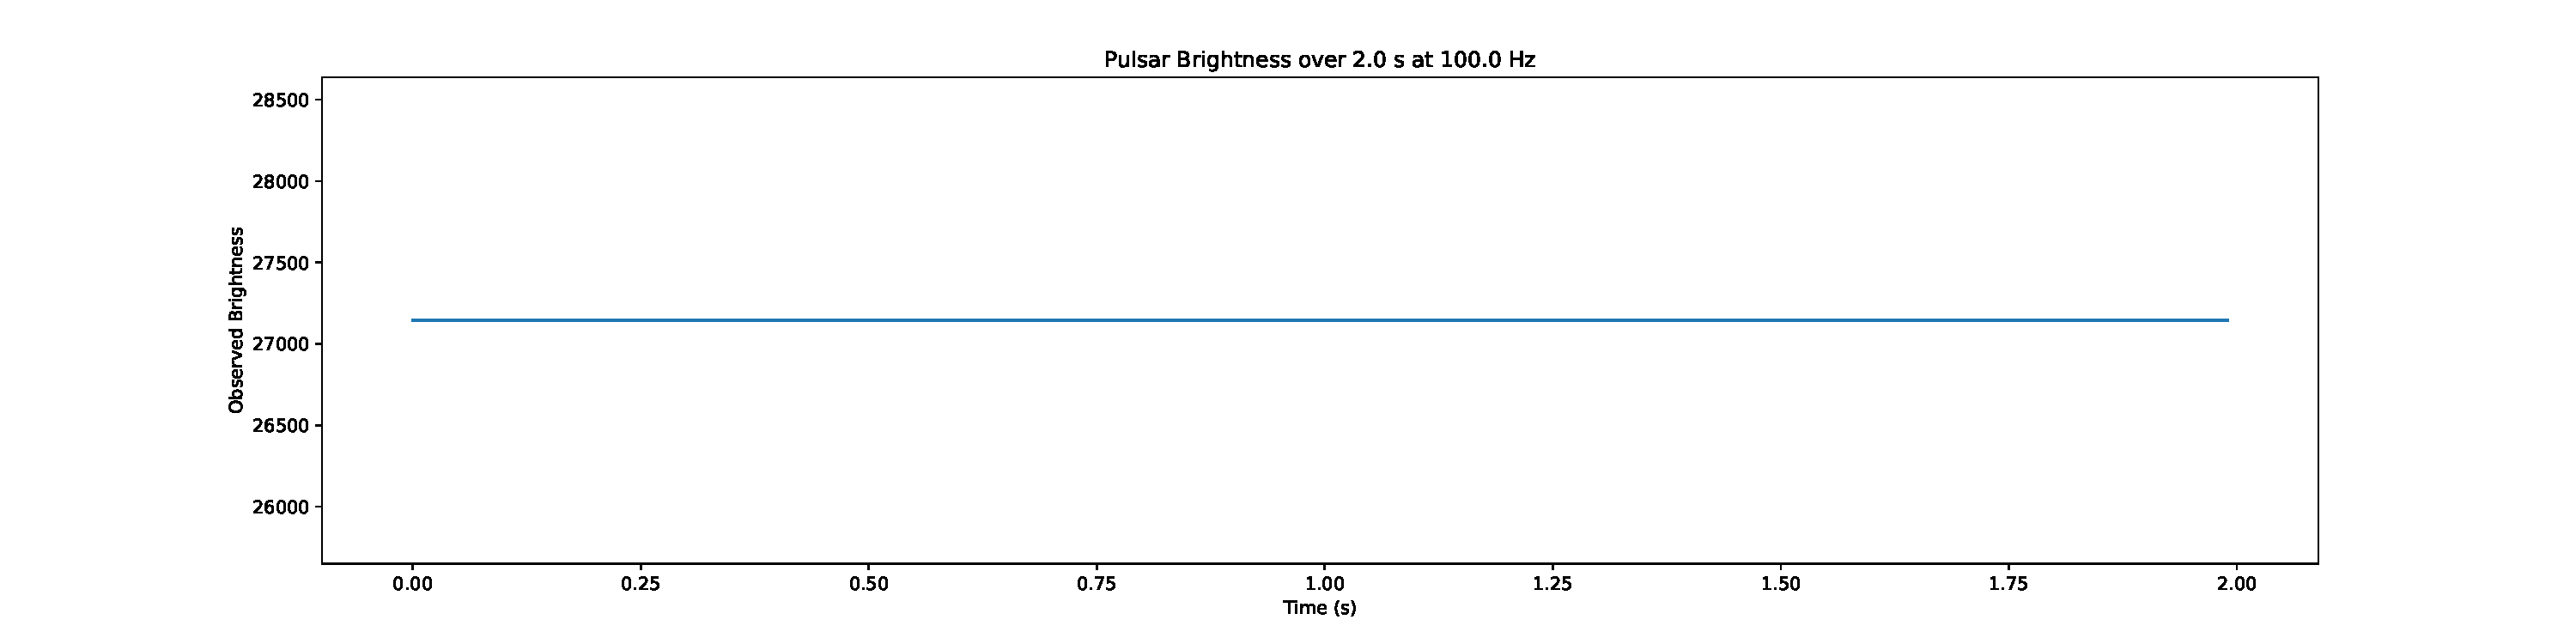
\includegraphics[width=\textwidth]{brightness_100.0_hz.pdf}

\section{Integrated Brightness}

Physical detectors operate at discreet time internals. The following plot shows
a integration of the brightness profile using a $\Delta t = 0.25 \, ms$ or
$4000\, Hz$, $4\times$ faster than the pulsar frequency.

The integrated data produces a more smooth transition between peaks and troughs.
The cost is more computation time used to calculate each data chunk.

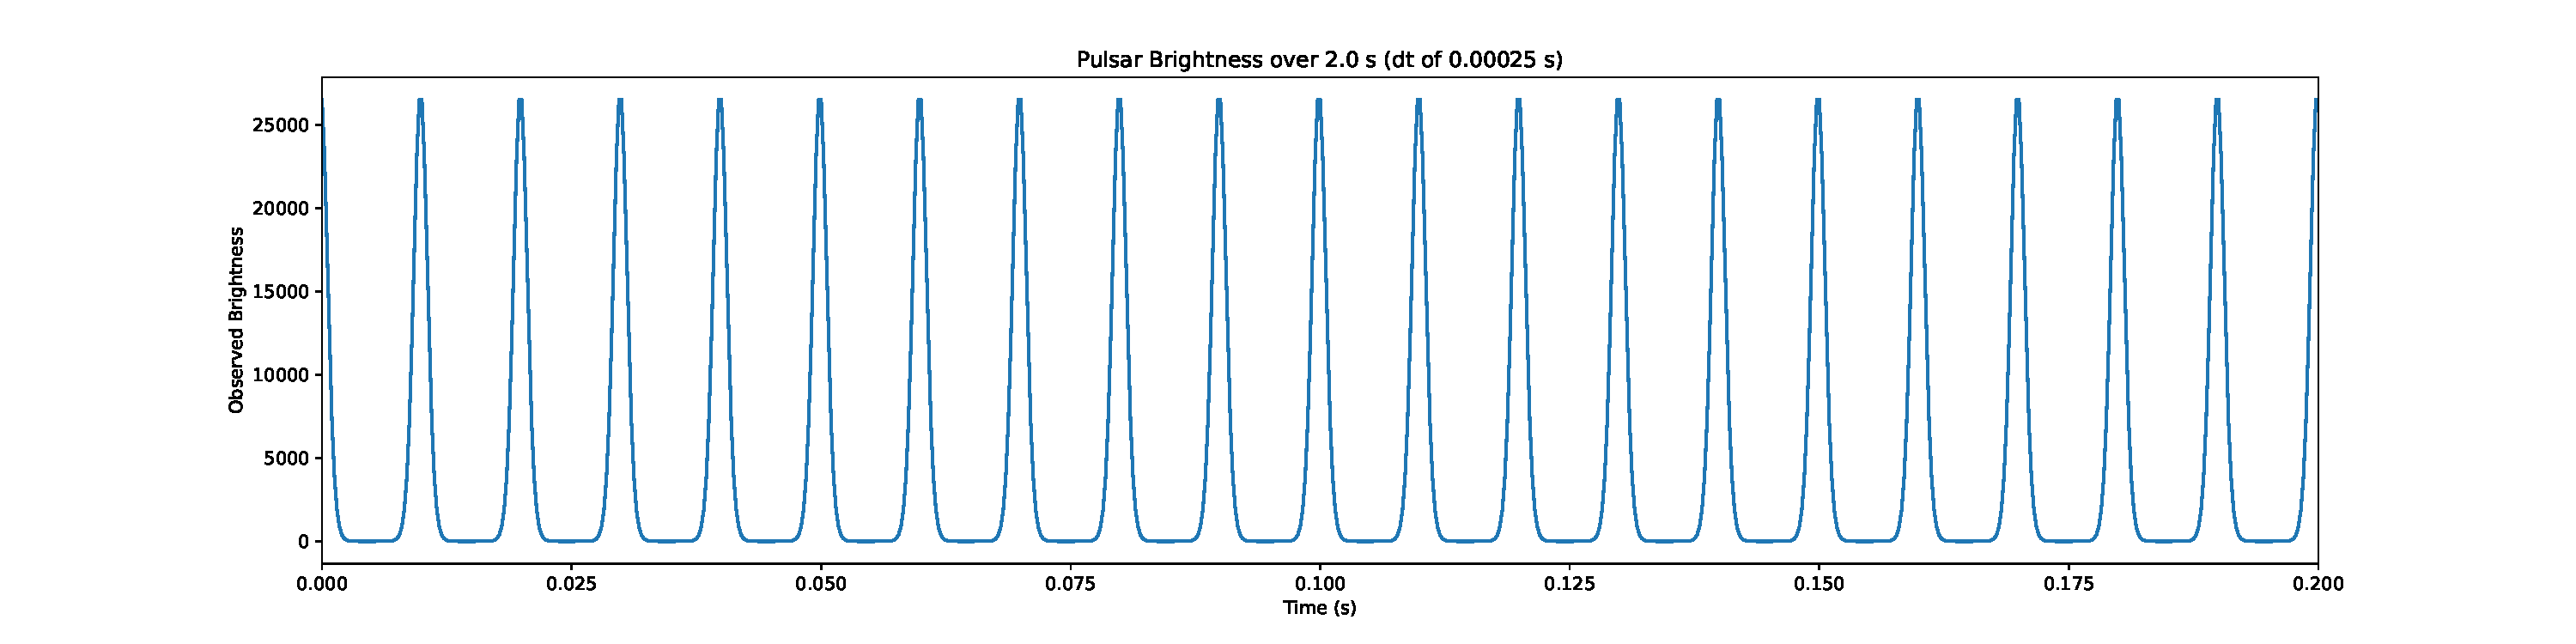
\includegraphics[width=\textwidth]{integrated_brightness.pdf}

\section{Adding noise}

Real data is also affected by noise. The next two plots show the same simulated
time series with a Gaussian noise with a standard deviation of 20\% the peak
observed brightness.

Although the frequency of pulses remains the same, the overall data trend is
less clear and a peak brightness cannot be directly inferred.

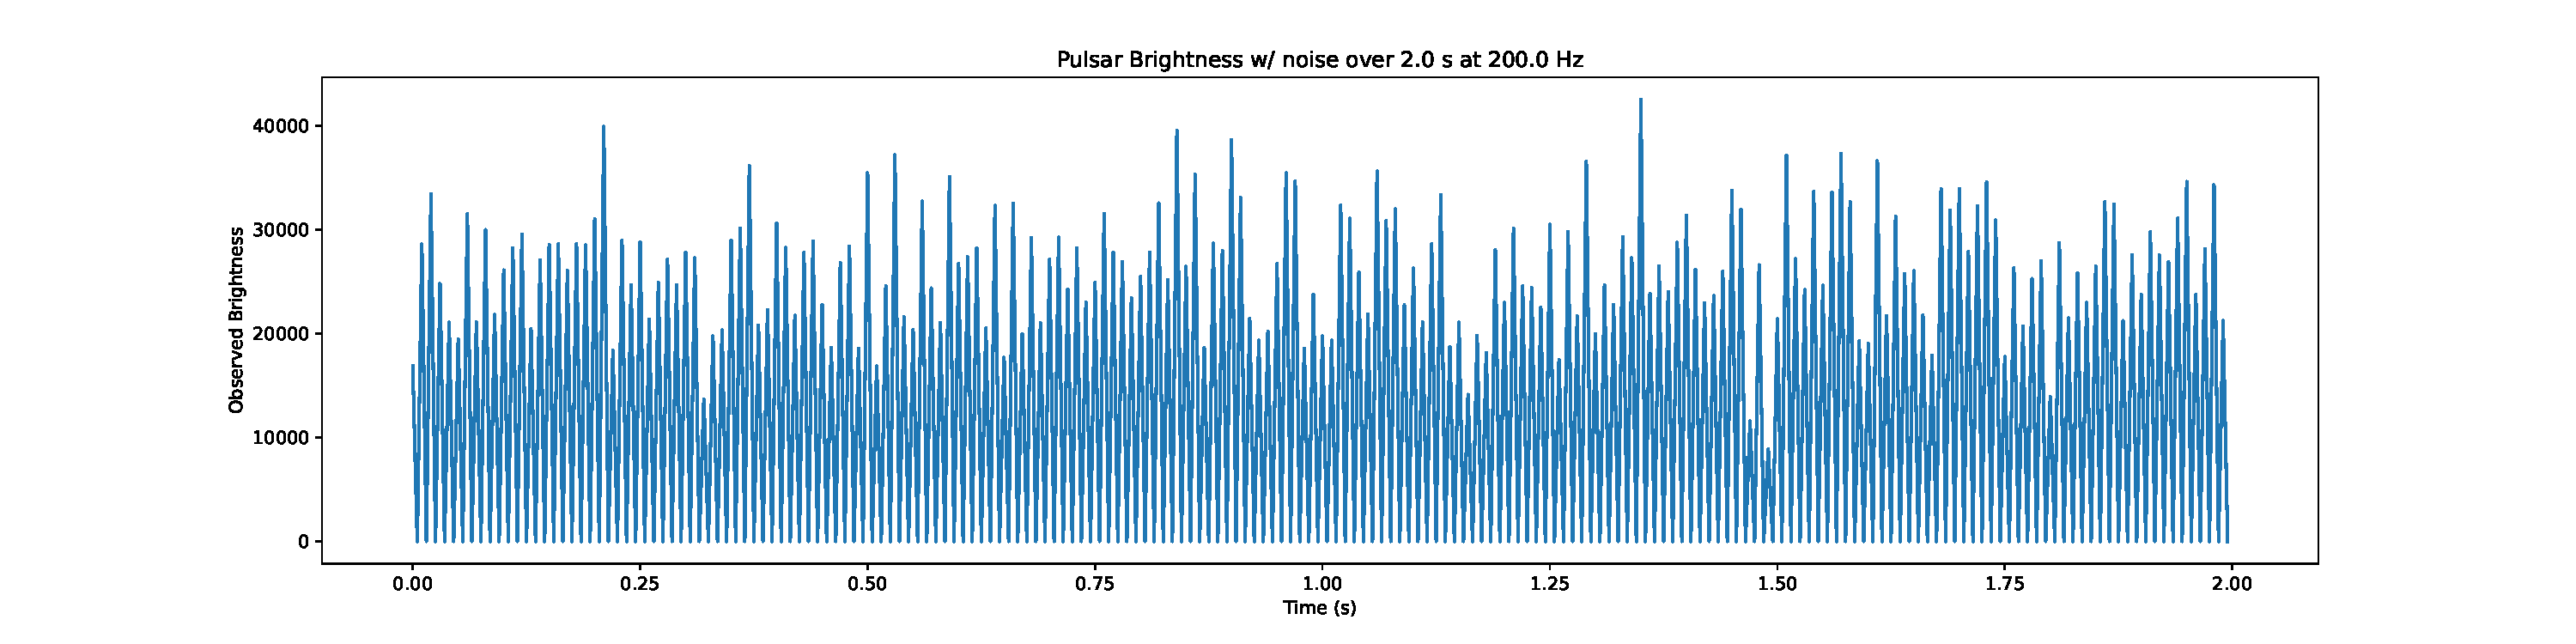
\includegraphics[width=\textwidth]{noise_brightness_200.0_hz.pdf}
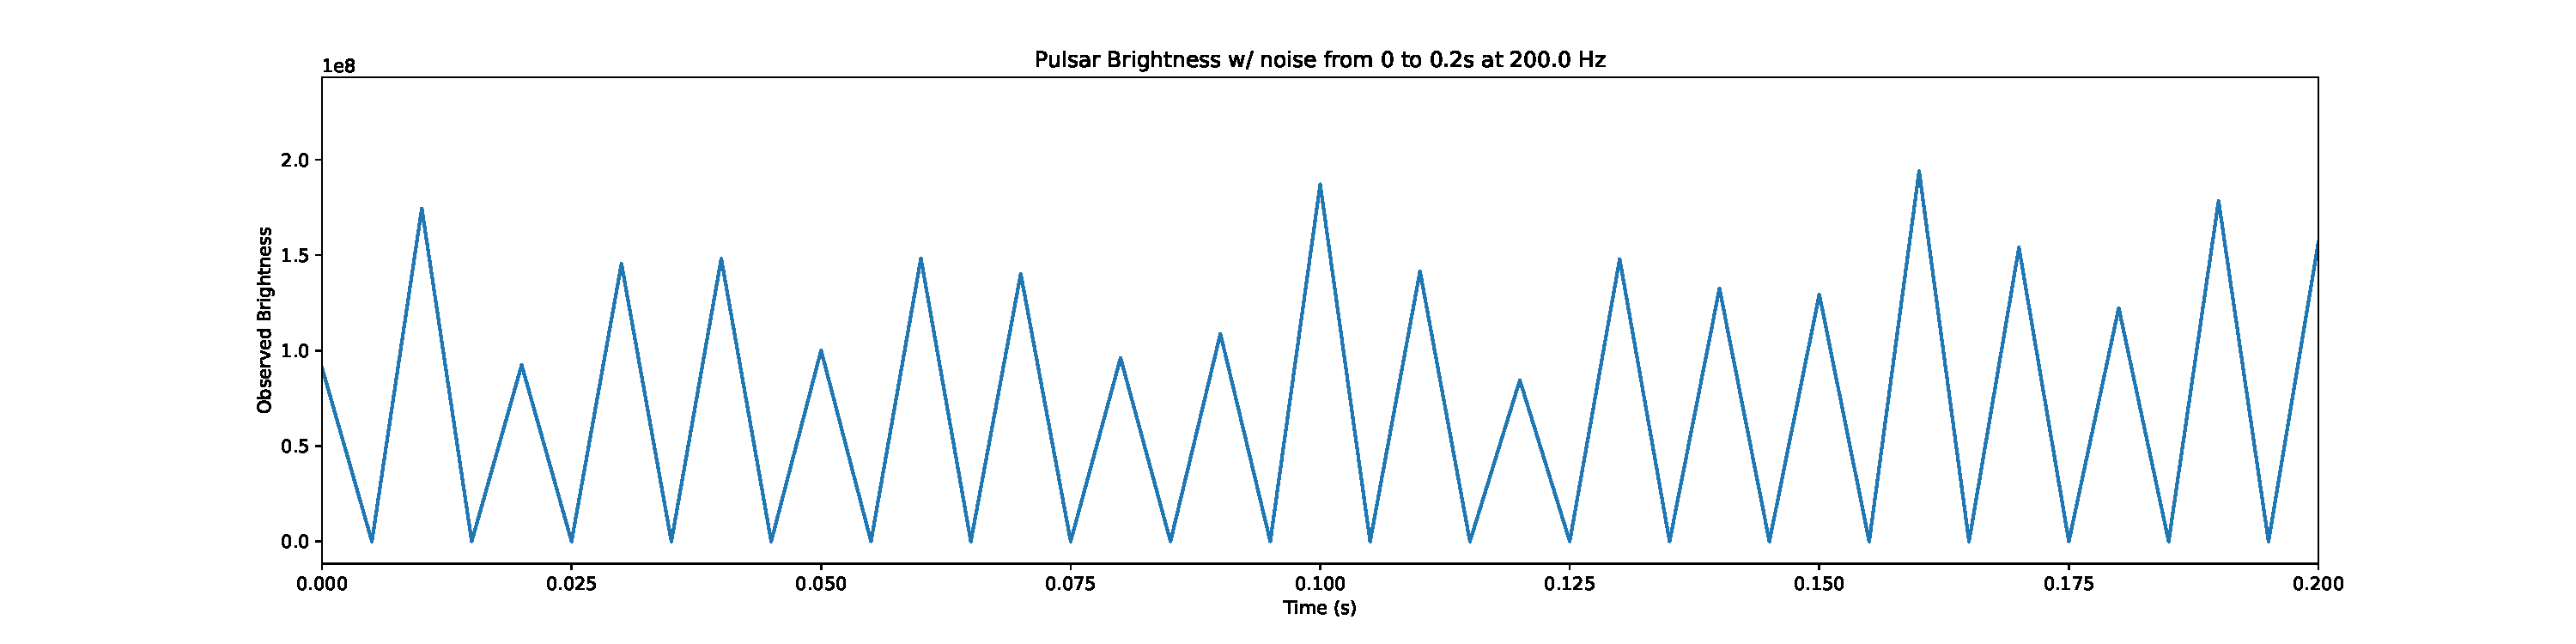
\includegraphics[width=\textwidth]{noise_brightness_200.0_hz_range.pdf}

\subsection{Search templates}

With the simulated profile with noise above, we can then generate different
profiles by varying the integrated brightness function (D, $\omega$, $\phi$) and
try to reverse estimate their brightness.

We define a search template $T_k(D, \omega, \phi)$ as:

\begin{equation}
    T_k = I_k(I_{peak}=1)
\end{equation}

The following six profiles are defined:

\begin{align*}
    T_{0}(D = 0.2, \omega = 6.28 rad/s, \phi = \pi rad)\\
    T_{1}(D = 0.4, \omega = 2.51 rad/s, \phi = \frac{\pi}{2} rad)\\
    T_{2}(D = 0.8, \omega = 2 rad/s, \phi = \frac{\pi}{4} rad)\\
    T_{3}(D = 0.1, \omega = 628.32 rad/s, \phi = 1 rad)\\
    T_{4}(D = 0.12, \omega = 6283.19 rad/s, \phi = \frac{3 \pi}{4} rad)\\
    T_{5}(D = 0.16, \omega = 12.57 rad/s, \phi = 2 \pi rad)\\
\end{align*}

Where $T_{3}$ contains the original values for the simulation.

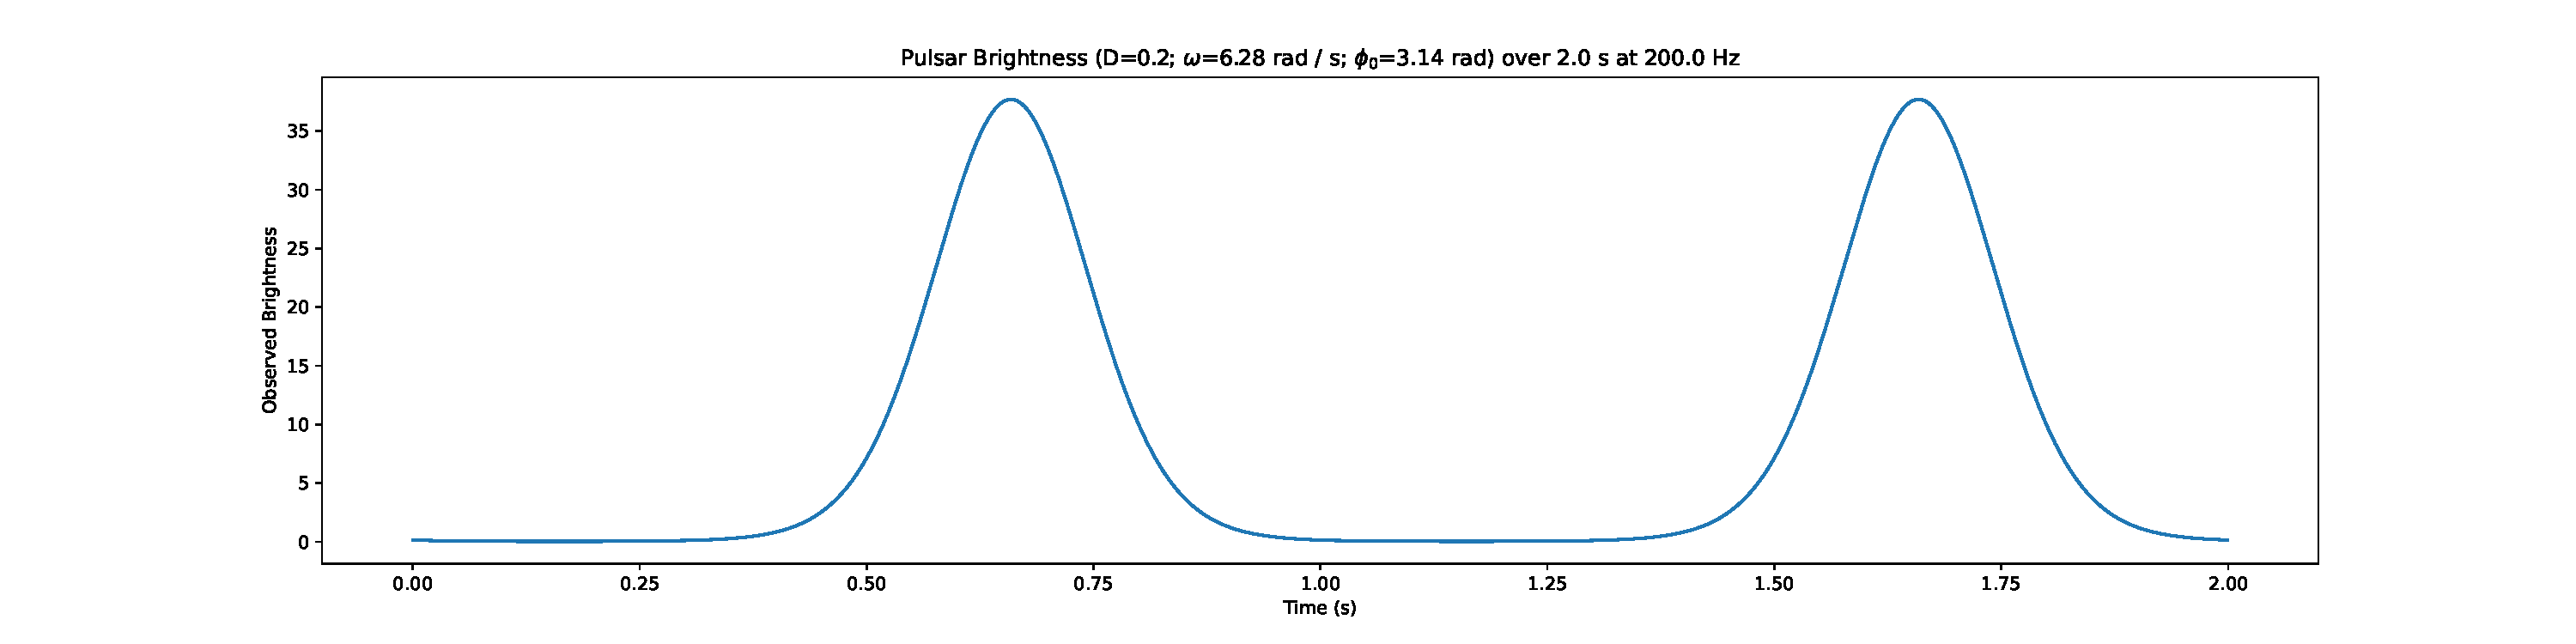
\includegraphics[width=\textwidth]{search_template_brightness_0.pdf}
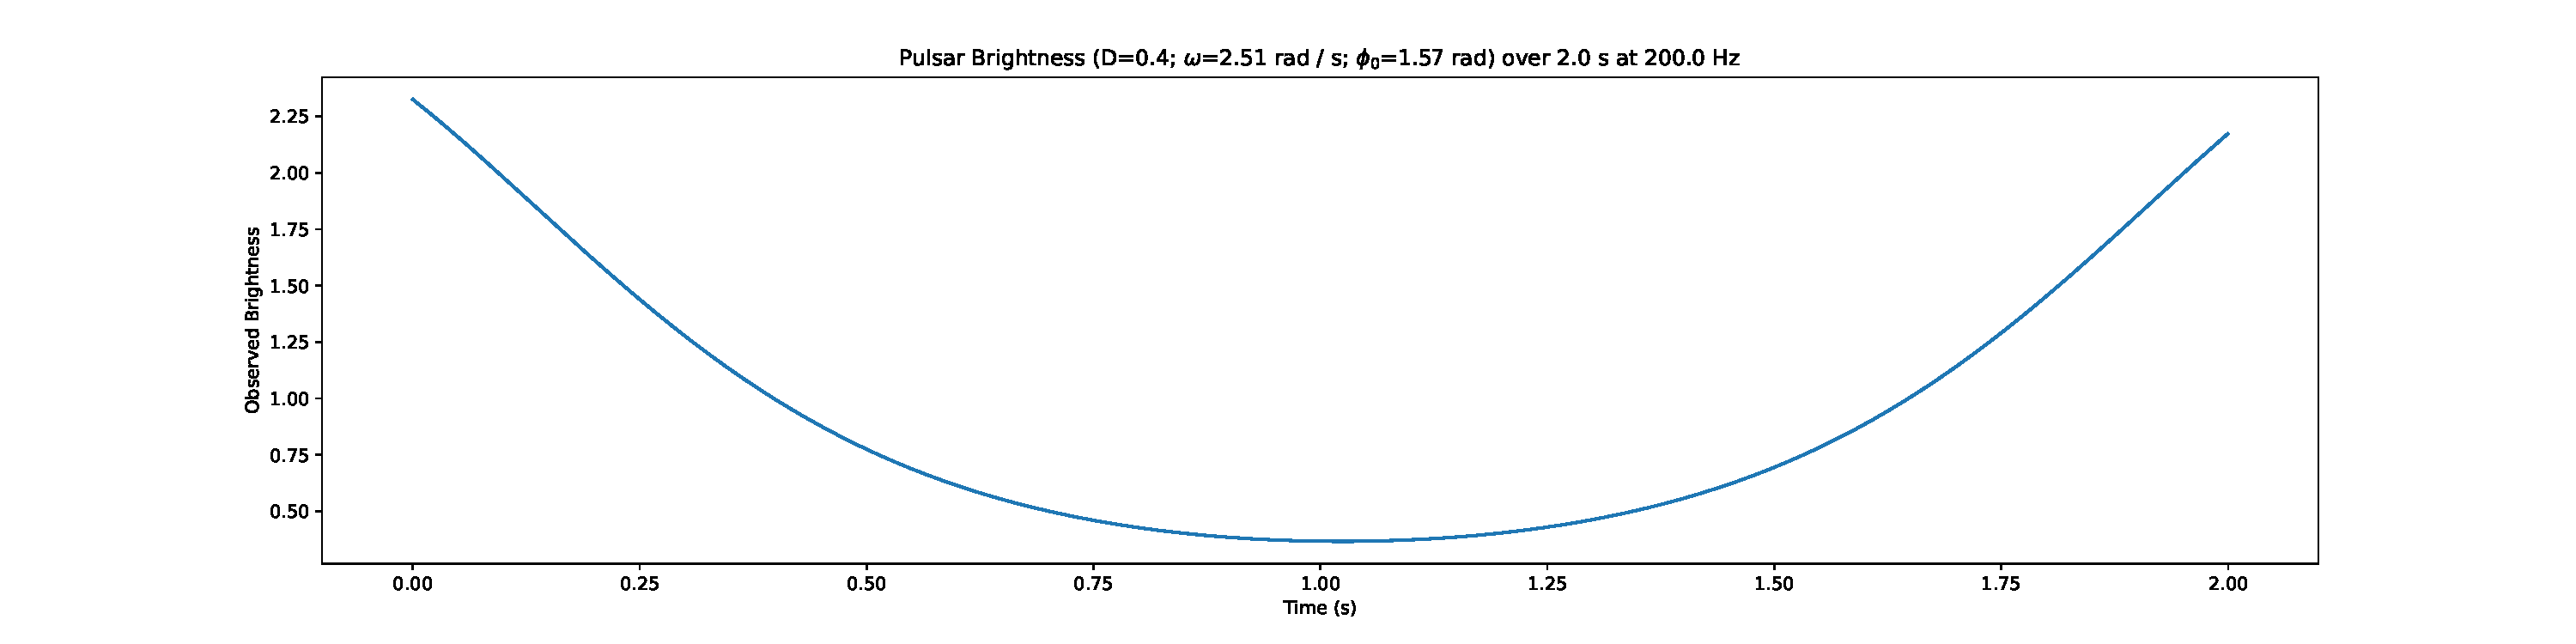
\includegraphics[width=\textwidth]{search_template_brightness_1.pdf}
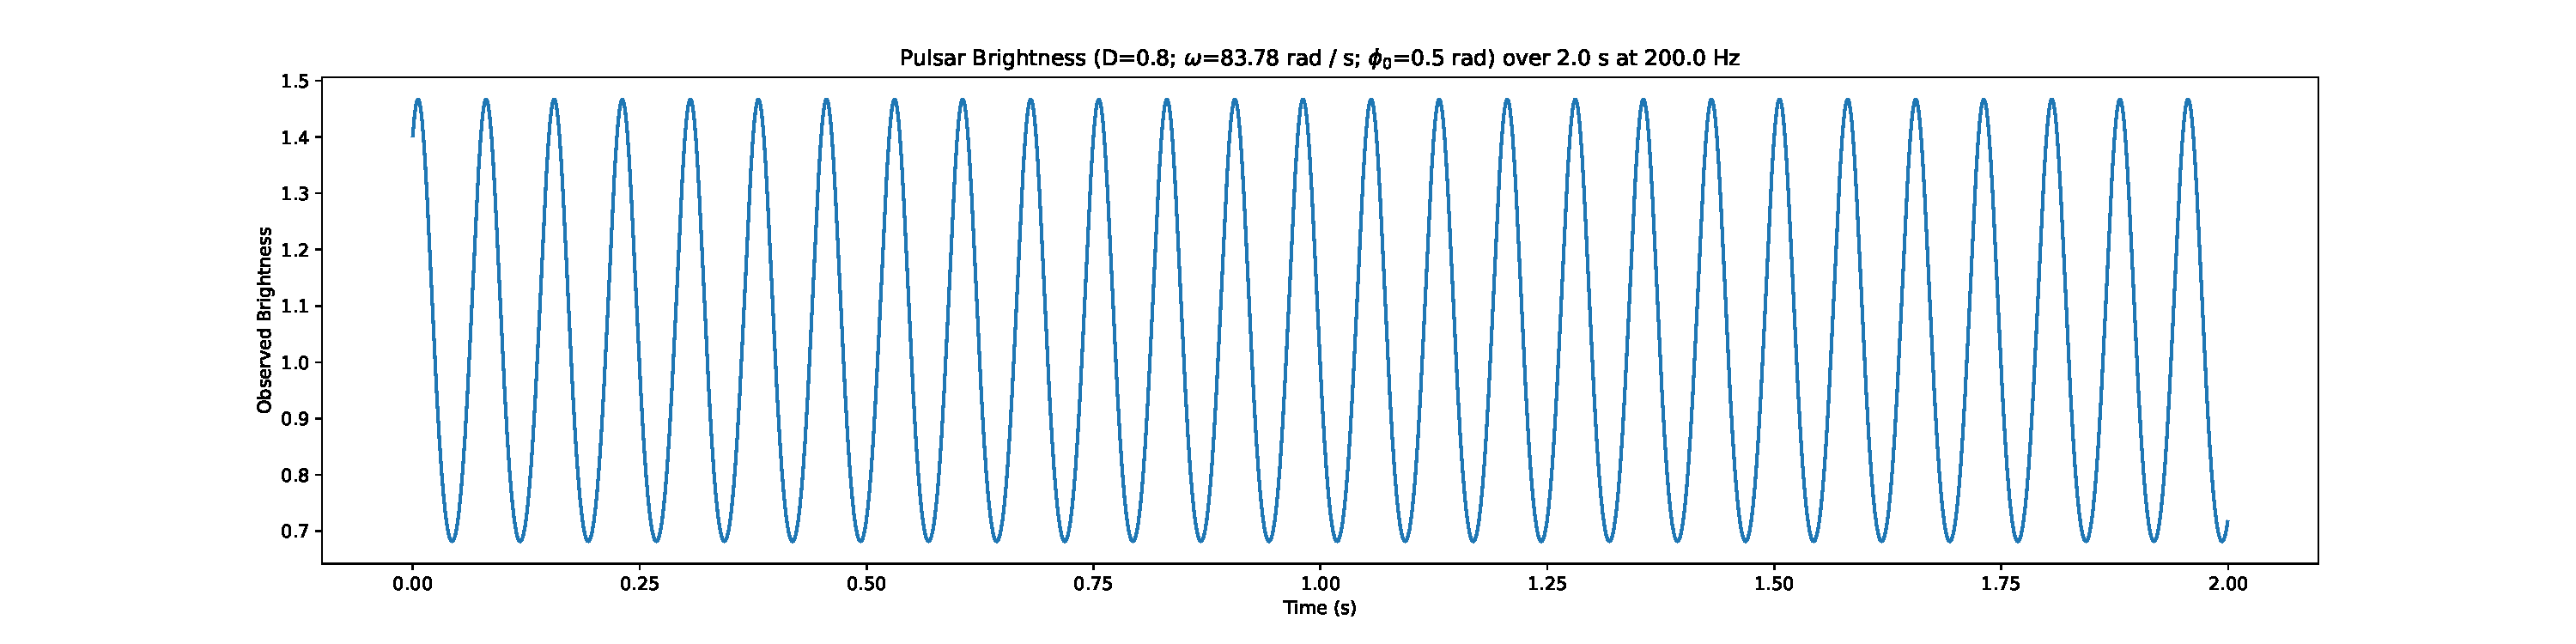
\includegraphics[width=\textwidth]{search_template_brightness_2.pdf}
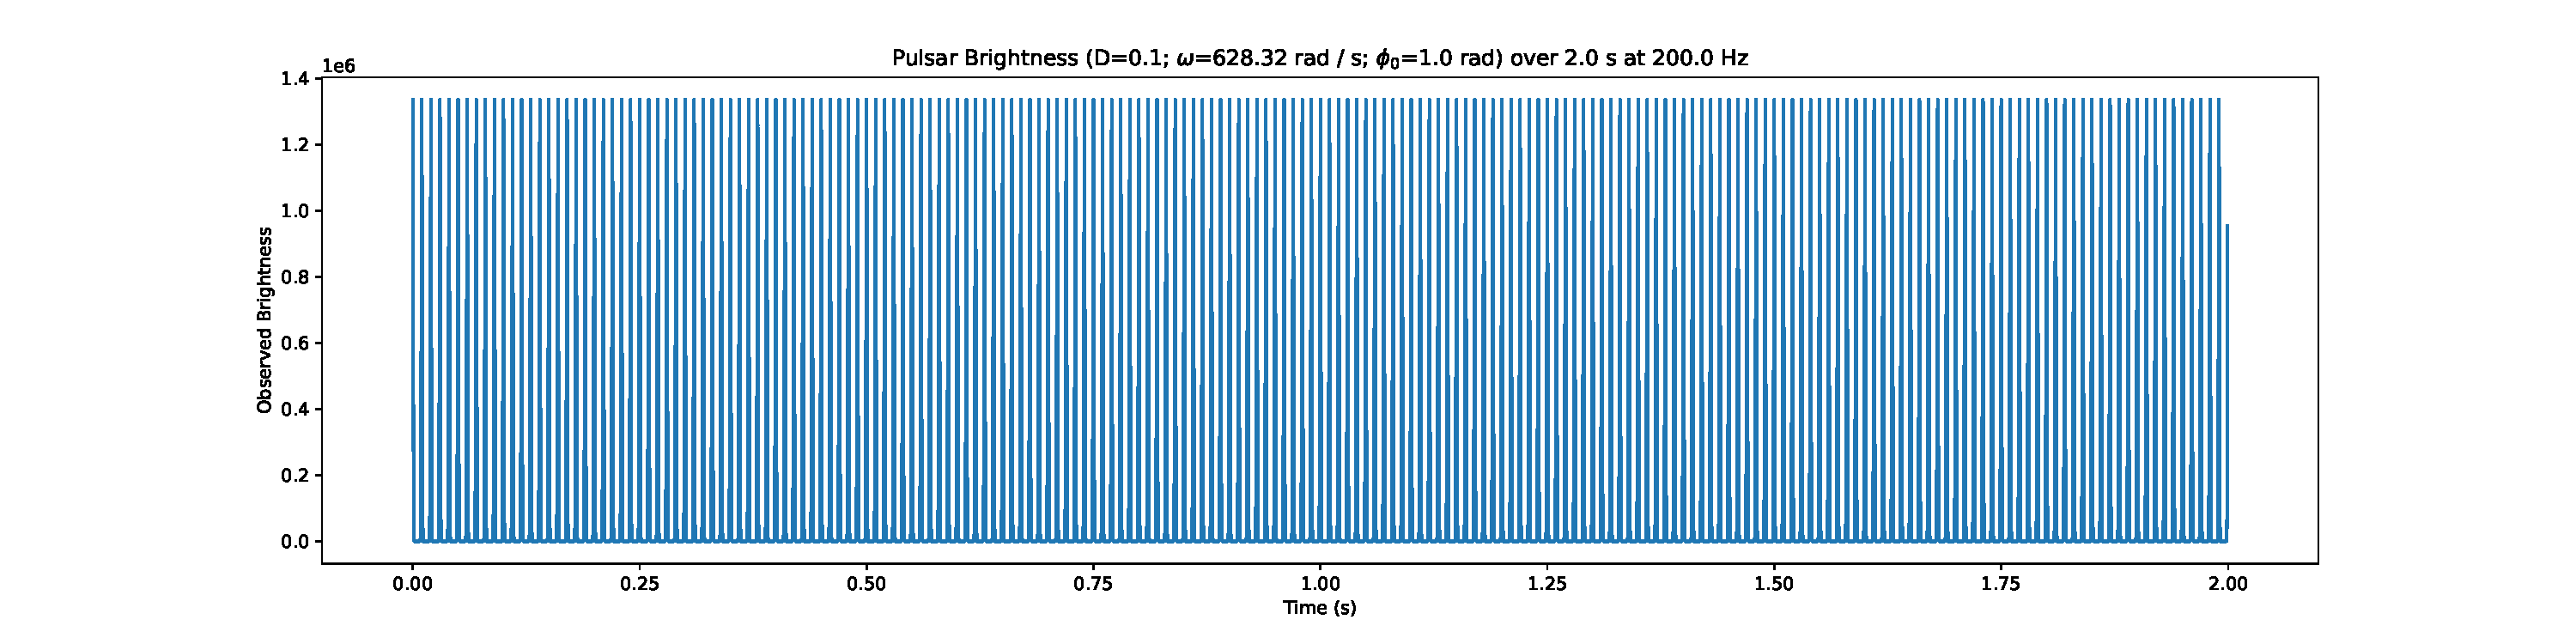
\includegraphics[width=\textwidth]{search_template_brightness_3.pdf}
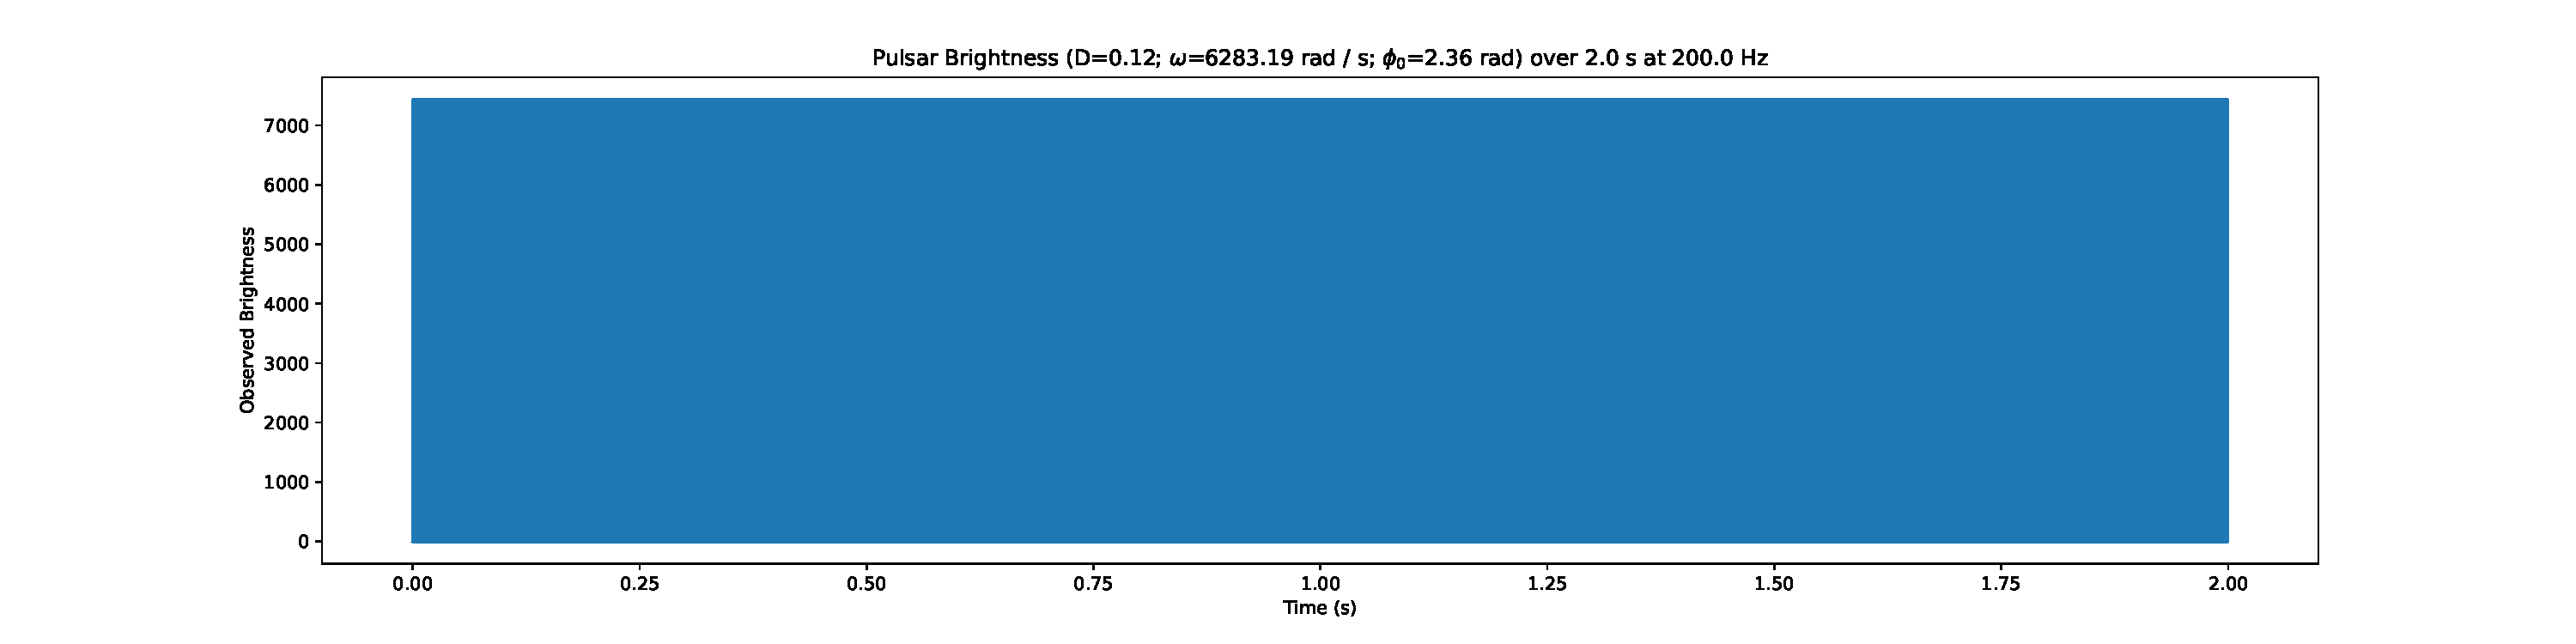
\includegraphics[width=\textwidth]{search_template_brightness_4.pdf}
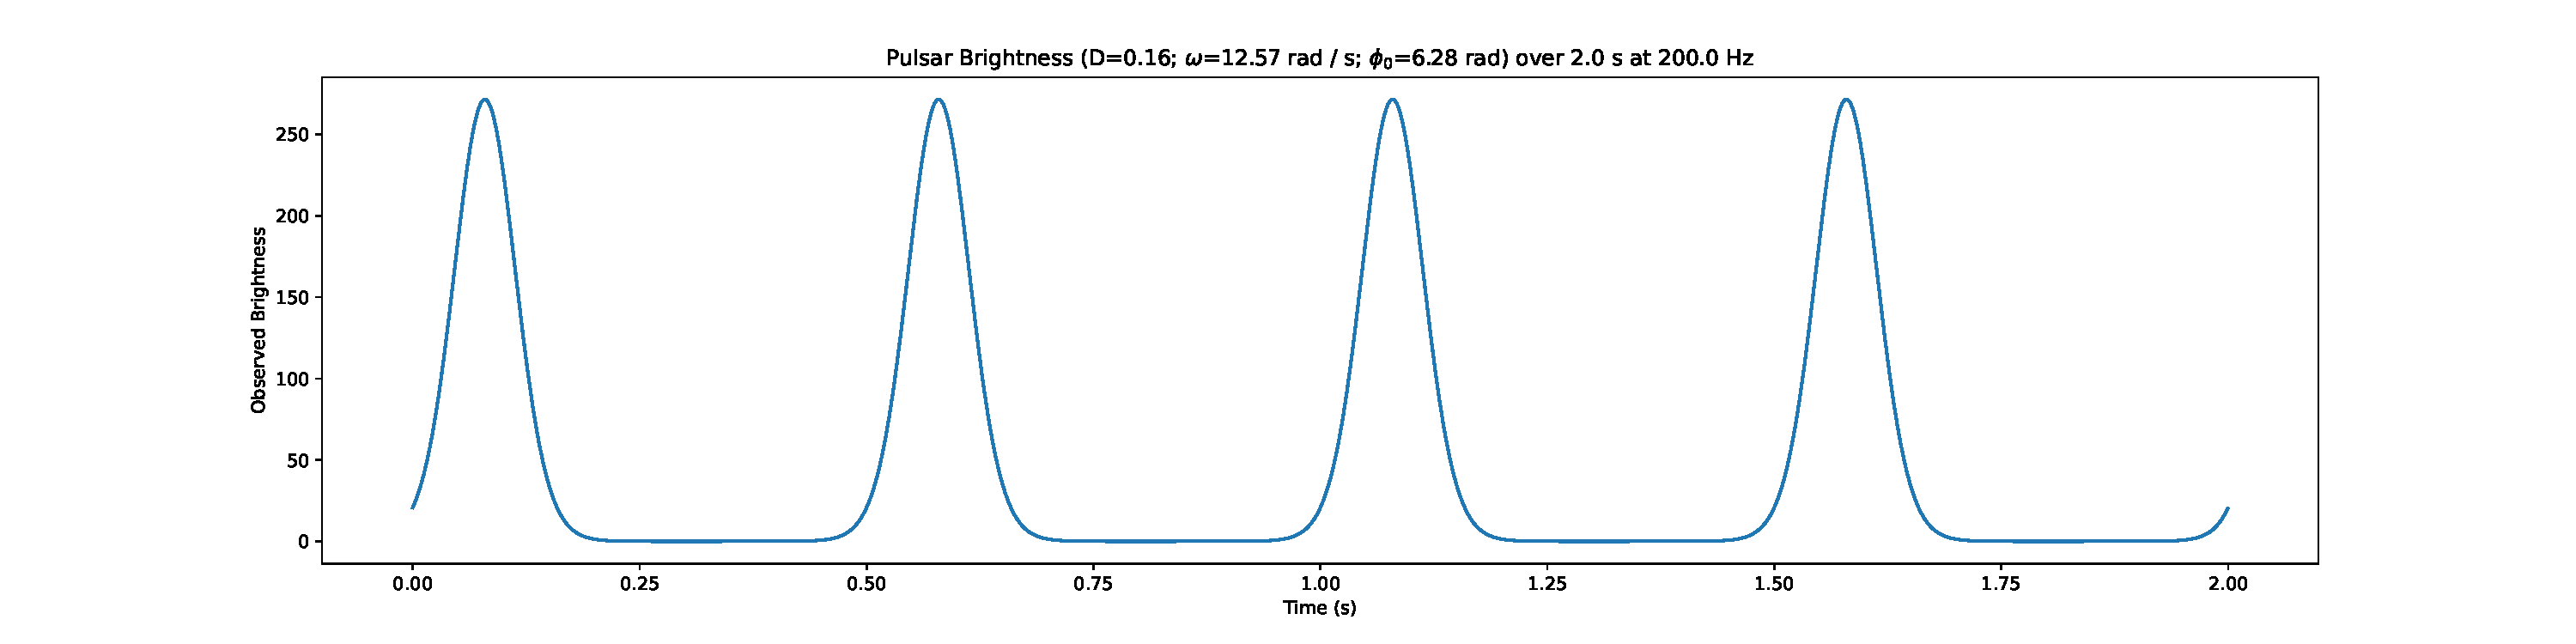
\includegraphics[width=\textwidth]{search_template_brightness_5.pdf}

\section{Brightness Estimator}

The following brightness estimators were found for each template:

\begin{align*}
    \hat{I}_{peak} & T_{0} = 183.18\\
    & T_{1} = 3646.38\\
    & T_{2} = 4310.19\\
    & T_{3} = 0.0231\\
    & T_{4} = 0.7605\\
    & T_{5} = 24.710\\
\end{align*}

Template $T_{3}$, the original value, should have had the brightness estimator closer to the $I_{peak}$, but this relationship was not found with the current implementation.

\section{Conclusion}

I need to better understand linear regression before a proper conclusion can be obtained. To that extend, the following weeks of the SURP project will provide more time for further research and inquiry about linear regression.

\section{References}

Grafarend, E. \& Awange. J. (2012) Applications of Linear and Nonlinear Models:
Fixed Effects, Random Effects. Springer Science \& Business Media, Aug 15.
(p. 362)

Henty, G., Paik, HJ. Distribution of Pulsar Duty Cycles. Nature 224, 1188–1189
(1969). https://doi.org/10.1038/2241188a0



\end{document}
